\documentclass[hyperref=colorlinks]{beamer}
\mode<presentation>
\usetheme{iclpt}
\setbeamertemplate{navigation symbols}{}
\setbeamertemplate{headline}{
\begin{beamercolorbox}[leftskip=.2cm,rightskip=.2cm,topskip=.2cm,ht=1.1cm,dp=0.1cm,wd=\textwidth]{institute in head/foot}
  
\includegraphics[height=1cm]{icl.pdf}
  \hfill
  
\includegraphics[height=1cm]{../Pics/CMS-Color.pdf}
\end{beamercolorbox}
}
\setbeamertemplate{footline}{
\begin{beamercolorbox}[ht=.55cm,dp=0.4cm,wd=\textwidth,leftskip=.3cm]{author in head/foot}%
  \begin{minipage}[c]{5cm}%
    \usebeamerfont{author in head/foot}
    \insertshortauthor 
    \insertshorttitle
    \end{minipage}\hfill%
  \insertframenumber{} / \pageref{lastframe}
  \hfill
  \begin{minipage}{6cm}
    \hfill
  \end{minipage}
\end{beamercolorbox}%
}

\usepackage{color}
\usepackage{tabularx,colortbl}
\usepackage{graphicx}
\usepackage{pdfpages}
\usepackage{feynmp}
\usepackage{multirow}
\DeclareGraphicsRule{*}{mps}{*}{}

\title{\vspace{-0.2cm} Higgs to Invisible MC Comparison}
%\subtitle{This result: HIG-15-012 \\ Contributing analyses: HIG-13-030, HIG-14-038, EXO-12-055}
%\author[P. Dunne]{\underline{P. Dunne} on behalf of the H$\rightarrow$invisible analysis group}
\titlegraphic{
  \vspace{-0.7cm}
  %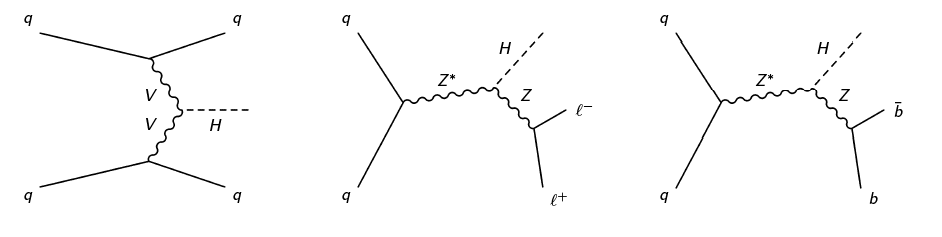
\includegraphics[width=\textwidth]{TalkPics/invcomb021213/feyndiags}
%% \begin{fmfgraph*}(100,70)
%%         \fmfleft{i1,i2}
%%         \fmfright{o1,o2,o3}
%%         \fmf{fermion}{i1,v1,o1}
%%         \fmf{fermion}{i2,v2,o3}
%%         \fmf{phantom,tension=4/5}{v1,v2}
%%         \fmffreeze
%%         \fmf{photon,label=$W,,Z$}{v1,v3}
%%         \fmf{photon,label=$W,,Z$}{v2,v3}
%%         \fmf{dashes}{v3,o2}
%%         \fmflabel{$q$}{i1}
%%         \fmflabel{$q$}{i2}
%%         \fmflabel{$q$}{o1}
%%         \fmflabel{$q$}{o3}
%%         \fmflabel{$H$}{o2}
%%       \end{fmfgraph*}
}
\date{}
\begin{document}
\begin{fmffile}{phenoplots141015feyndiags}

%TITLE PAGE
\section{Title}
\begin{frame}
  \titlepage
  
\end{frame}

\begin{frame}
  \frametitle{Introduction}
  \begin{block}{}
    \begin{itemize}
    \item We wanted to check if the differences seen between Madgraph+delphes and Powheg+CMS were from generator or reconstruction
    \item Powheg samples generated with the same config as the CMS samples have been processed with delphes
    \item We have used these samples to validate our delphes model
    \item[-] Powheg+CMS and Powheg+Delphes yields now match to 10\%
    \item Next check is Madgraph+delphes against Powheg+delphes
    \end{itemize}
  \end{block}
\end{frame}

%!!CLOSURE TEST STATEMENT PU jet ID
%OUTLINE
\begin{frame}
  \frametitle{Cut flow}
  \scriptsize
  \begin{block}{}
    \begin{itemize}
    \item Compare yields cut by cut (numbers shown are numbers of events)
    \item Start with $\eta_{j1}\cdot\eta_{j2}<0$, MET significance$>3$, $\Delta\eta_{jj}>3.6$, jet 1 $p_{T}>35$ GeV, jet 2 $p_{T}>35$ GeV, $M_{jj}>700$ GeV, trigger MET$>40$ GeV 
    \item[-] All variables at trigger threshold plus MET significance$>3$ for technical reasons
    \end{itemize}
    \centering
  \end{block}
  \begin{block}{}
    \begin{tabular}{|l|c|c|}
      \hline
      Cut added & Powheg + CMS & Powheg + Delphes \\
      \hline
      Start point & 1552 & 2311 \\
      jet 1 $p_{T}>50$ GeV, jet 2 $p_{T}>45$ GeV & 1203 & 1834 \\
      MET$>90$ GeV & 1170 & 1793 \\
      $M_{jj}>1200$ GeV & 412 & 689 \\
      MET significance$>4$ & 315 & 519 \\
      min$\Delta\phi(j,MET)>2.3$ & 143 & 248 \\
      \hline
    \end{tabular}
  \end{block}
\end{frame}

\begin{frame}
  \frametitle{Efficiencies}
  \scriptsize
  \begin{block}{}
    \begin{itemize}
    \item Compare efficiencies of last cut cut by cut (numbers shown are efficiencies)
    \item Start with $\eta_{j1}\cdot\eta_{j2}<0$, MET significance$>3$, $\Delta\eta_{jj}>3.6$, jet 1 $p_{T}>35$ GeV, jet 2 $p_{T}>35$ GeV, $M_{jj}>700$ GeV, trigger MET$>40$ GeV 
    \item[-] All variables at trigger threshold plus MET significance$>3$ for technical reasons
    \item Efficiencies are quite similar
    \item Implies events are already missing at start point
    \end{itemize}
    \centering
  \end{block}
  \begin{block}{}
    \begin{tabular}{|l|c|c|}
      \hline
      Cut added & Powheg + CMS & Powheg + Delphes \\
      \hline
      jet 1 $p_{T}>50$ GeV, jet 2 $p_{T}>45$ GeV & 0.78 & 0.79 \\
      MET$>90$ GeV & 0.97 & 0.98 \\
      $M_{jj}>1200$ GeV & 0.35 & 0.38 \\
      MET significance$>4$ & 0.76 & 0.75 \\
      min$\Delta\phi(j,MET)>2.3$ & 0.45 & 0.48 \\
      \hline
    \end{tabular}
  \end{block}
\end{frame}


\begin{frame}
  \frametitle{Compare Distributions}
  \scriptsize
  \begin{block}{}
    \begin{itemize}
    \item Use looser selection to look for differences in distributions between Powheg and Madgraph
    \item All plots are normalised to same number of events
    \item Selection: $\Delta\eta_{jj}>3.6$, jet 1/2 $p_{T}>35$ GeV, trigger MET$>$40 GeV, $\eta_{j1}\cdot\eta_{j2}<0$
    \item $M_{jj}$ lower in Madgraph, MET significance very similar
    \end{itemize}
  \end{block}
  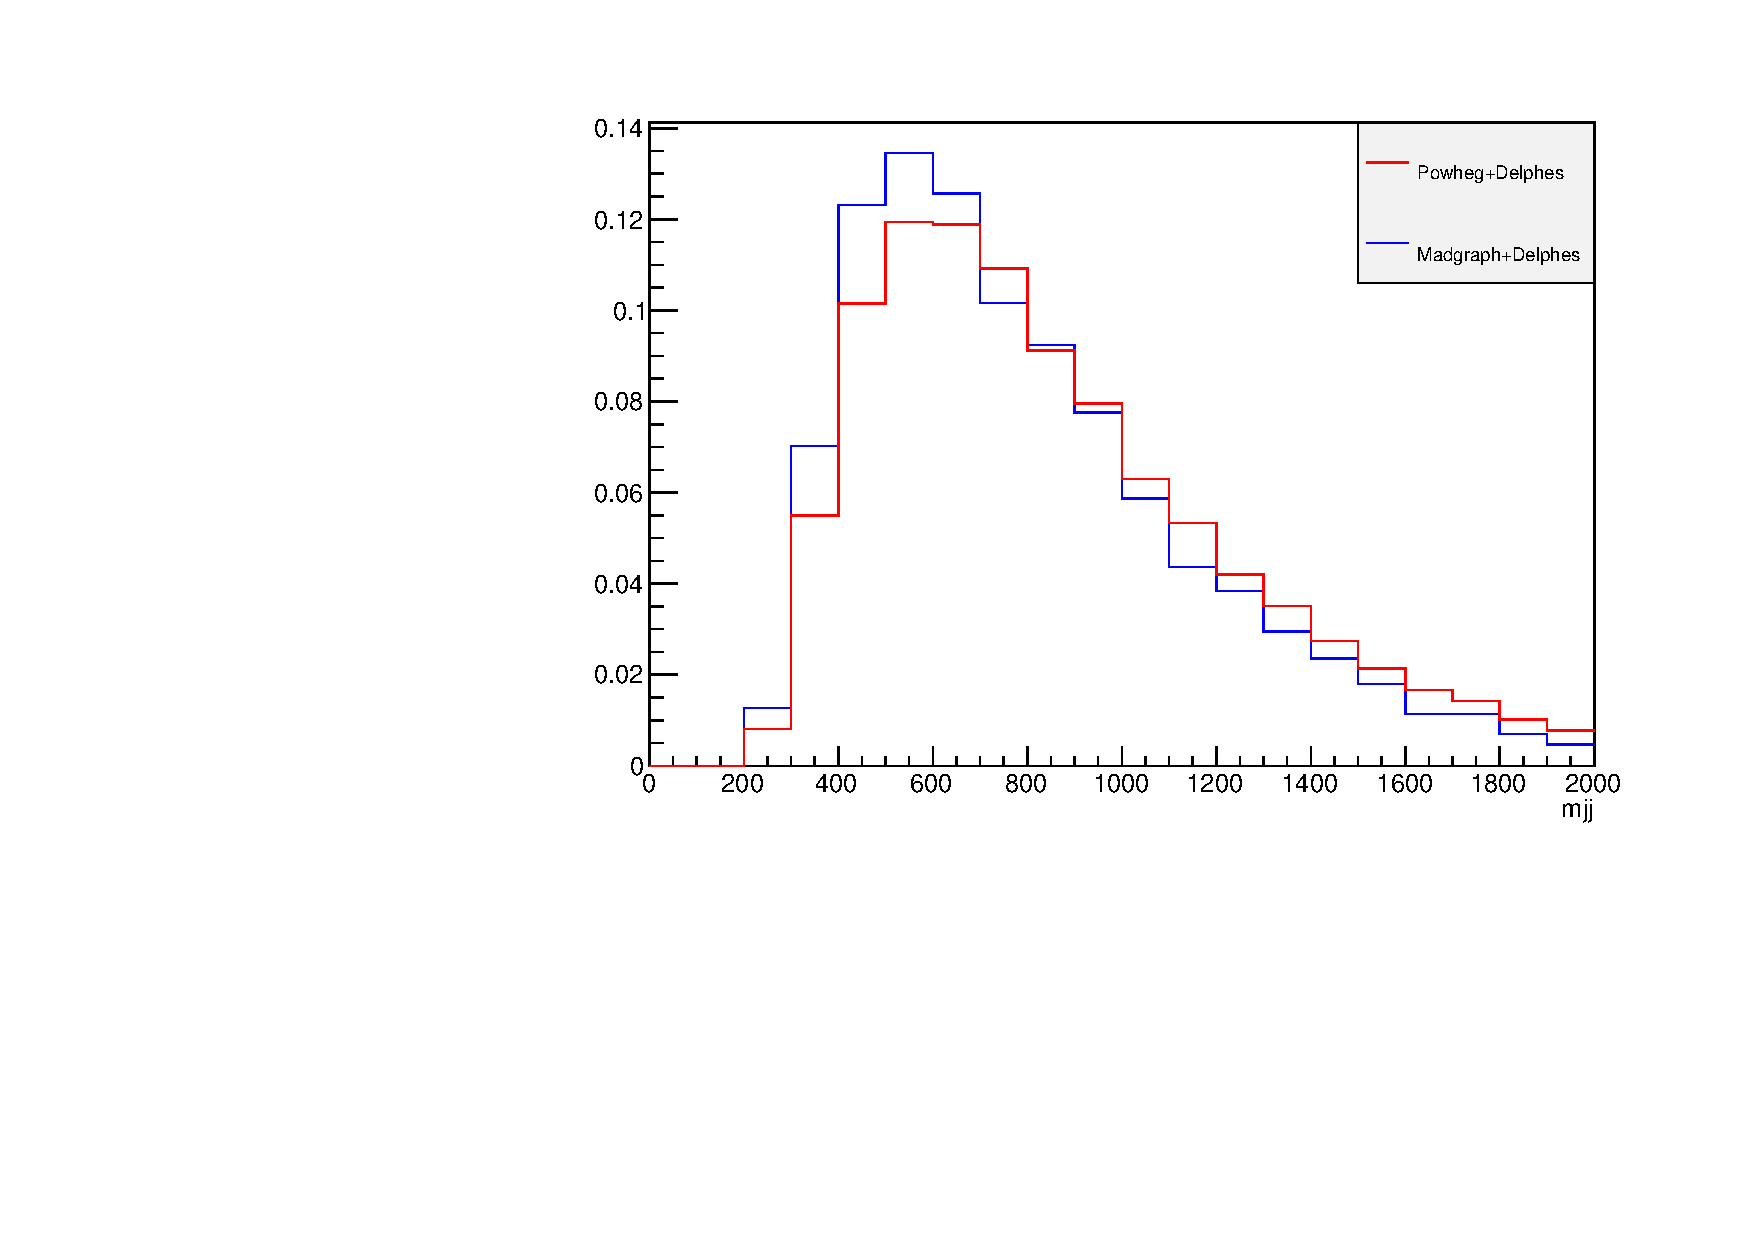
\includegraphics[width=.5\textwidth]{TalkPics/phenoplots221015/mjj_norm.pdf}
  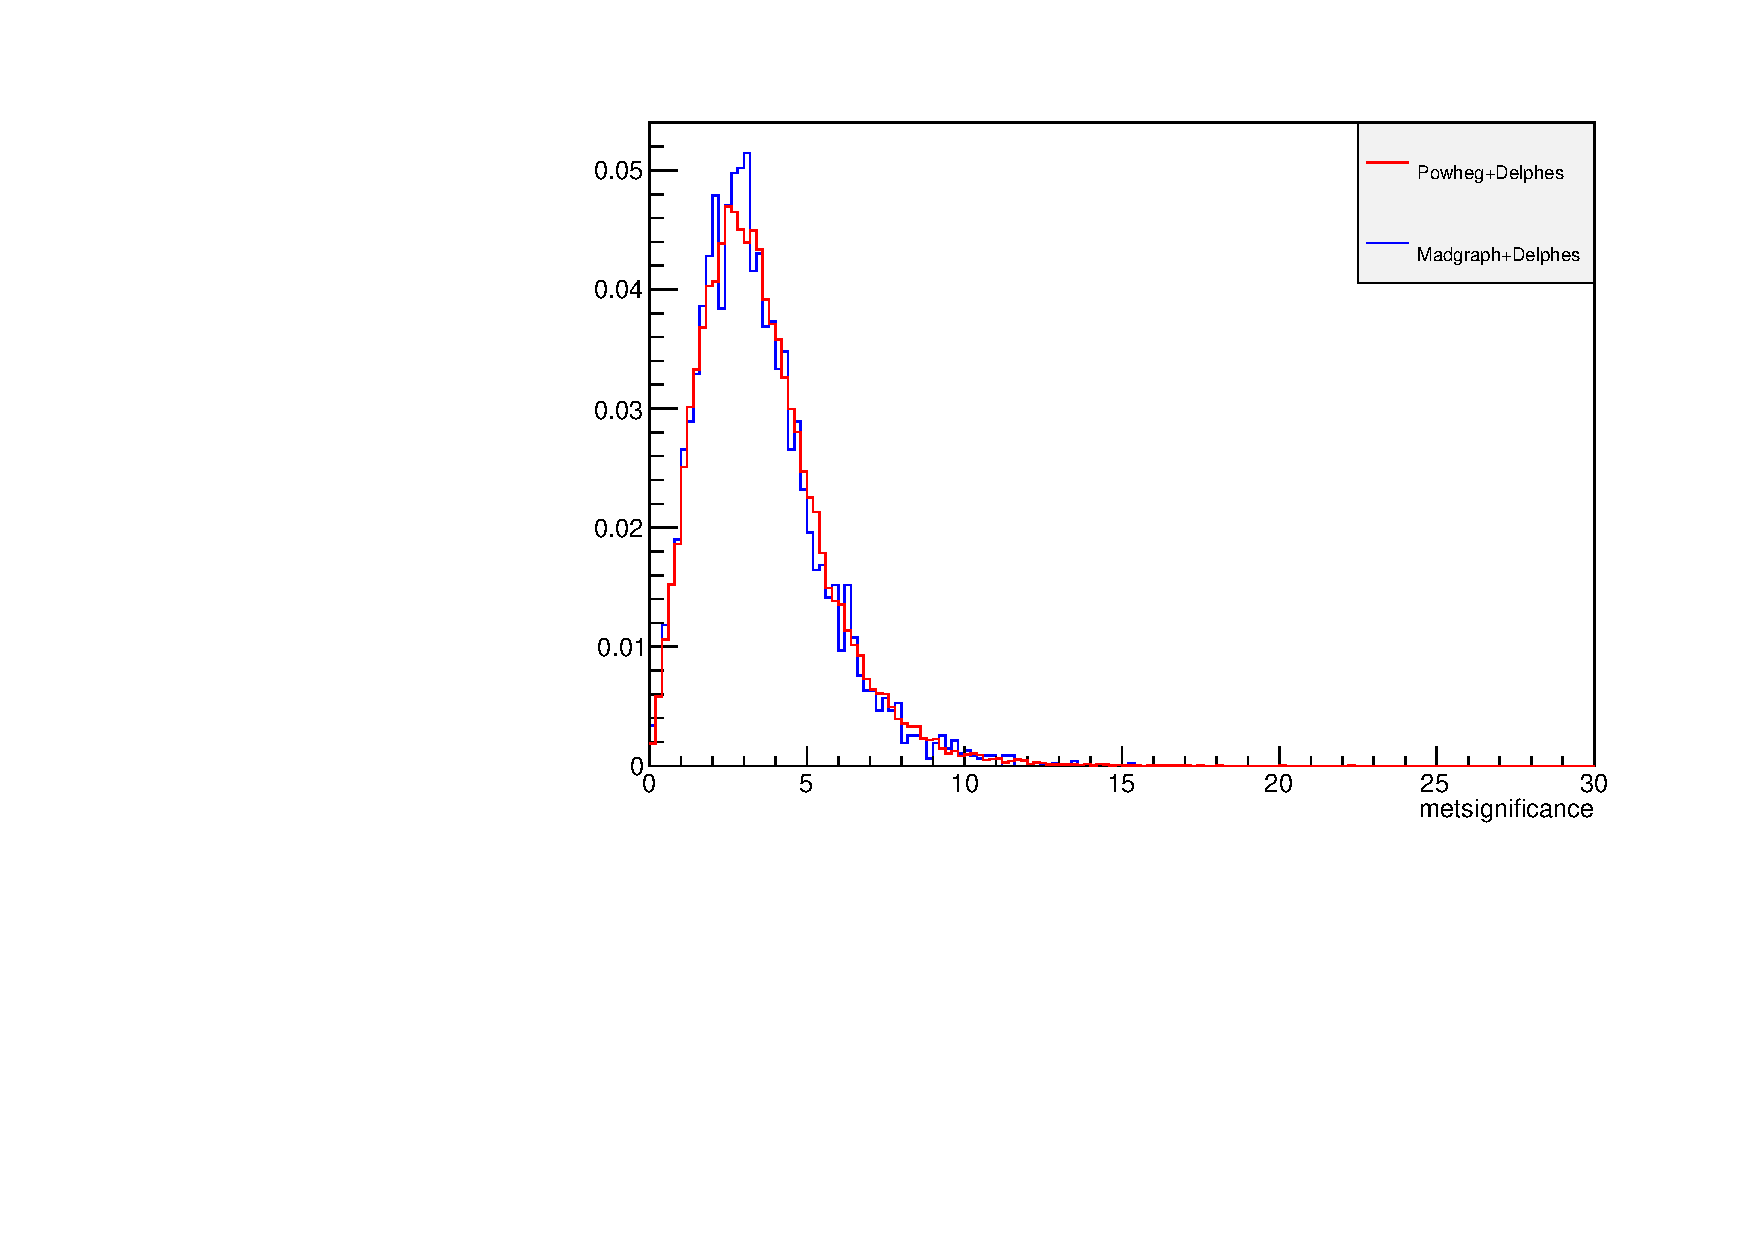
\includegraphics[width=.5\textwidth]{TalkPics/phenoplots221015/metsignificance_norm.pdf}
    
\end{frame}

\begin{frame}
  \frametitle{Compare Distributions}
  \scriptsize
  \begin{block}{}
    \begin{itemize}
    \item Selection: $\Delta\eta_{jj}>3.6$, jet 1/2 $p_{T}>35$ GeV, trigger MET$>$40 GeV, $\eta_{j1}\cdot\eta_{j2}<0$
    \item Jet pts lower in Madgraph
    \end{itemize}
  \end{block}
  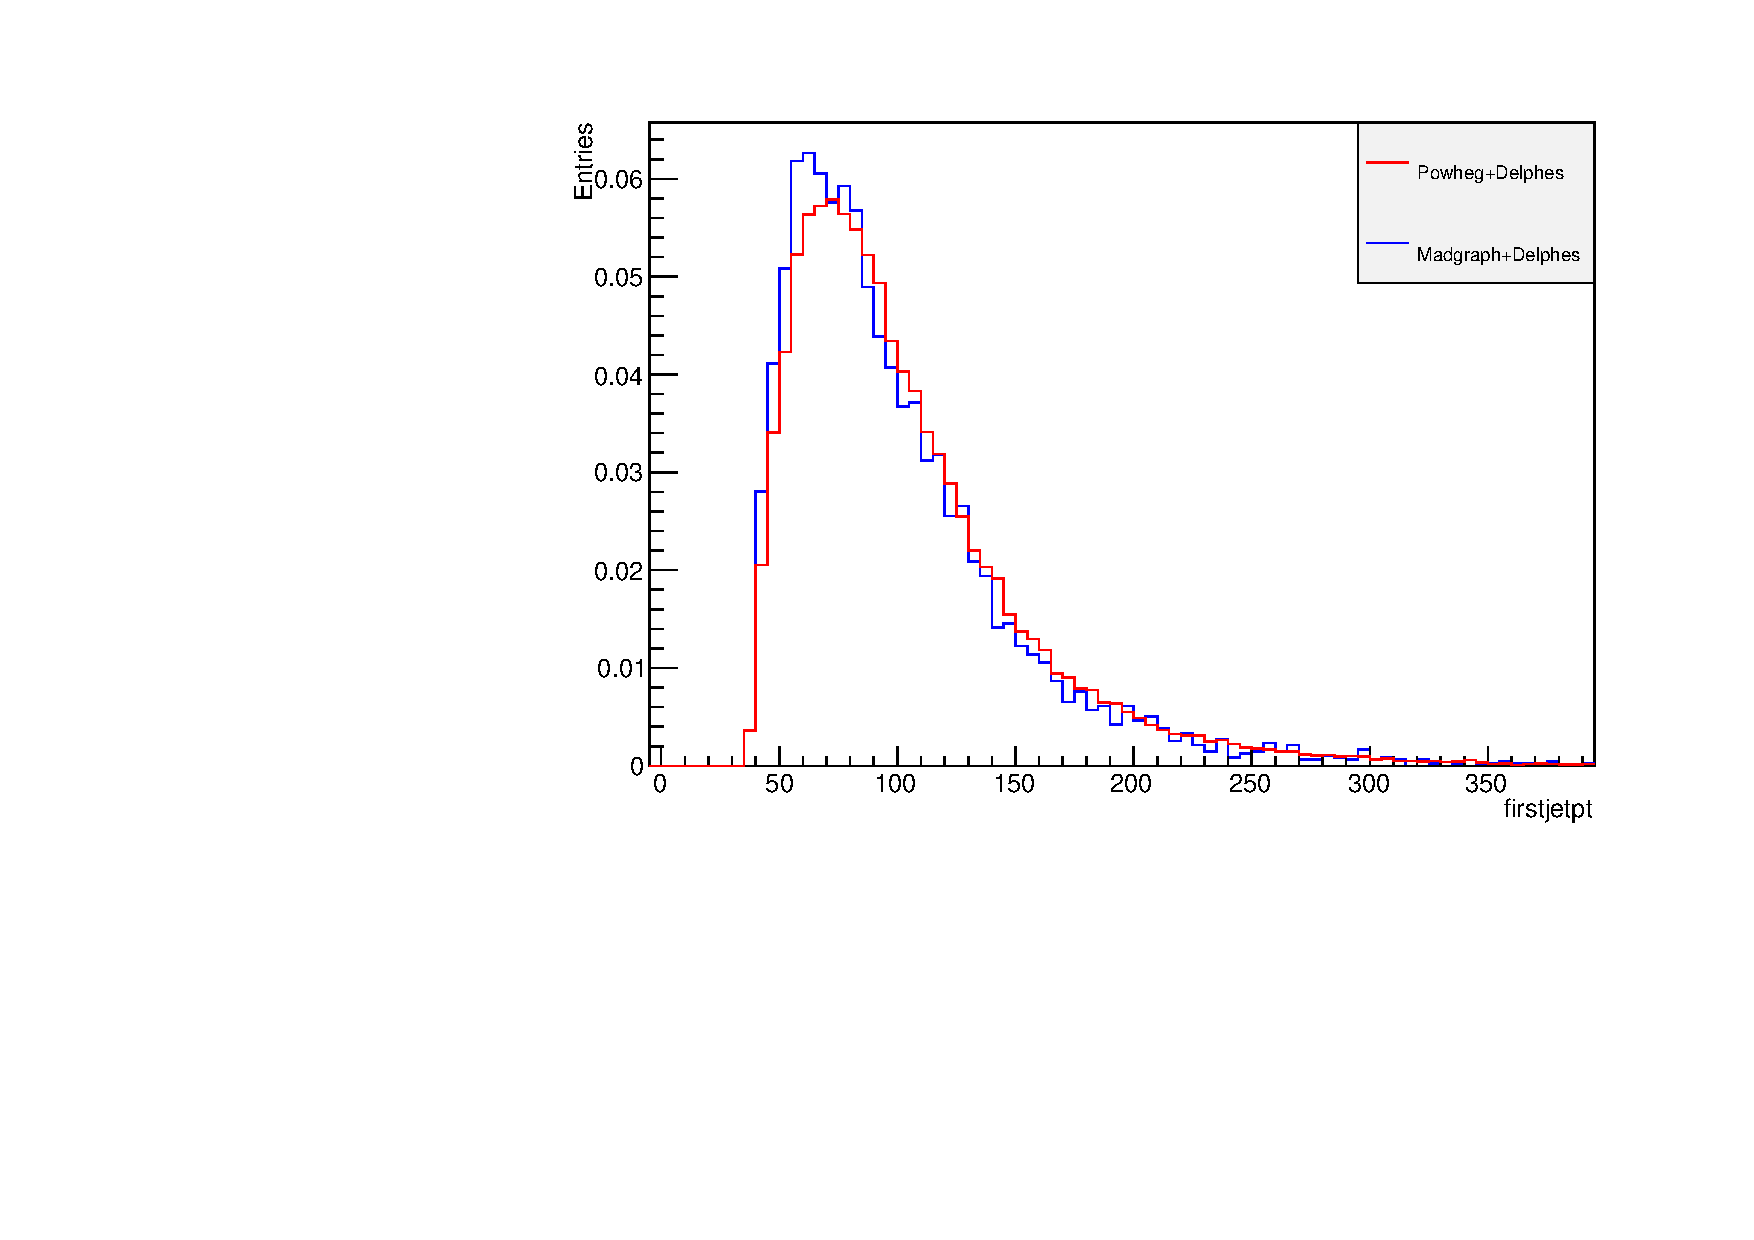
\includegraphics[width=.5\textwidth]{TalkPics/phenoplots221015/firstjetpt_norm.pdf}
  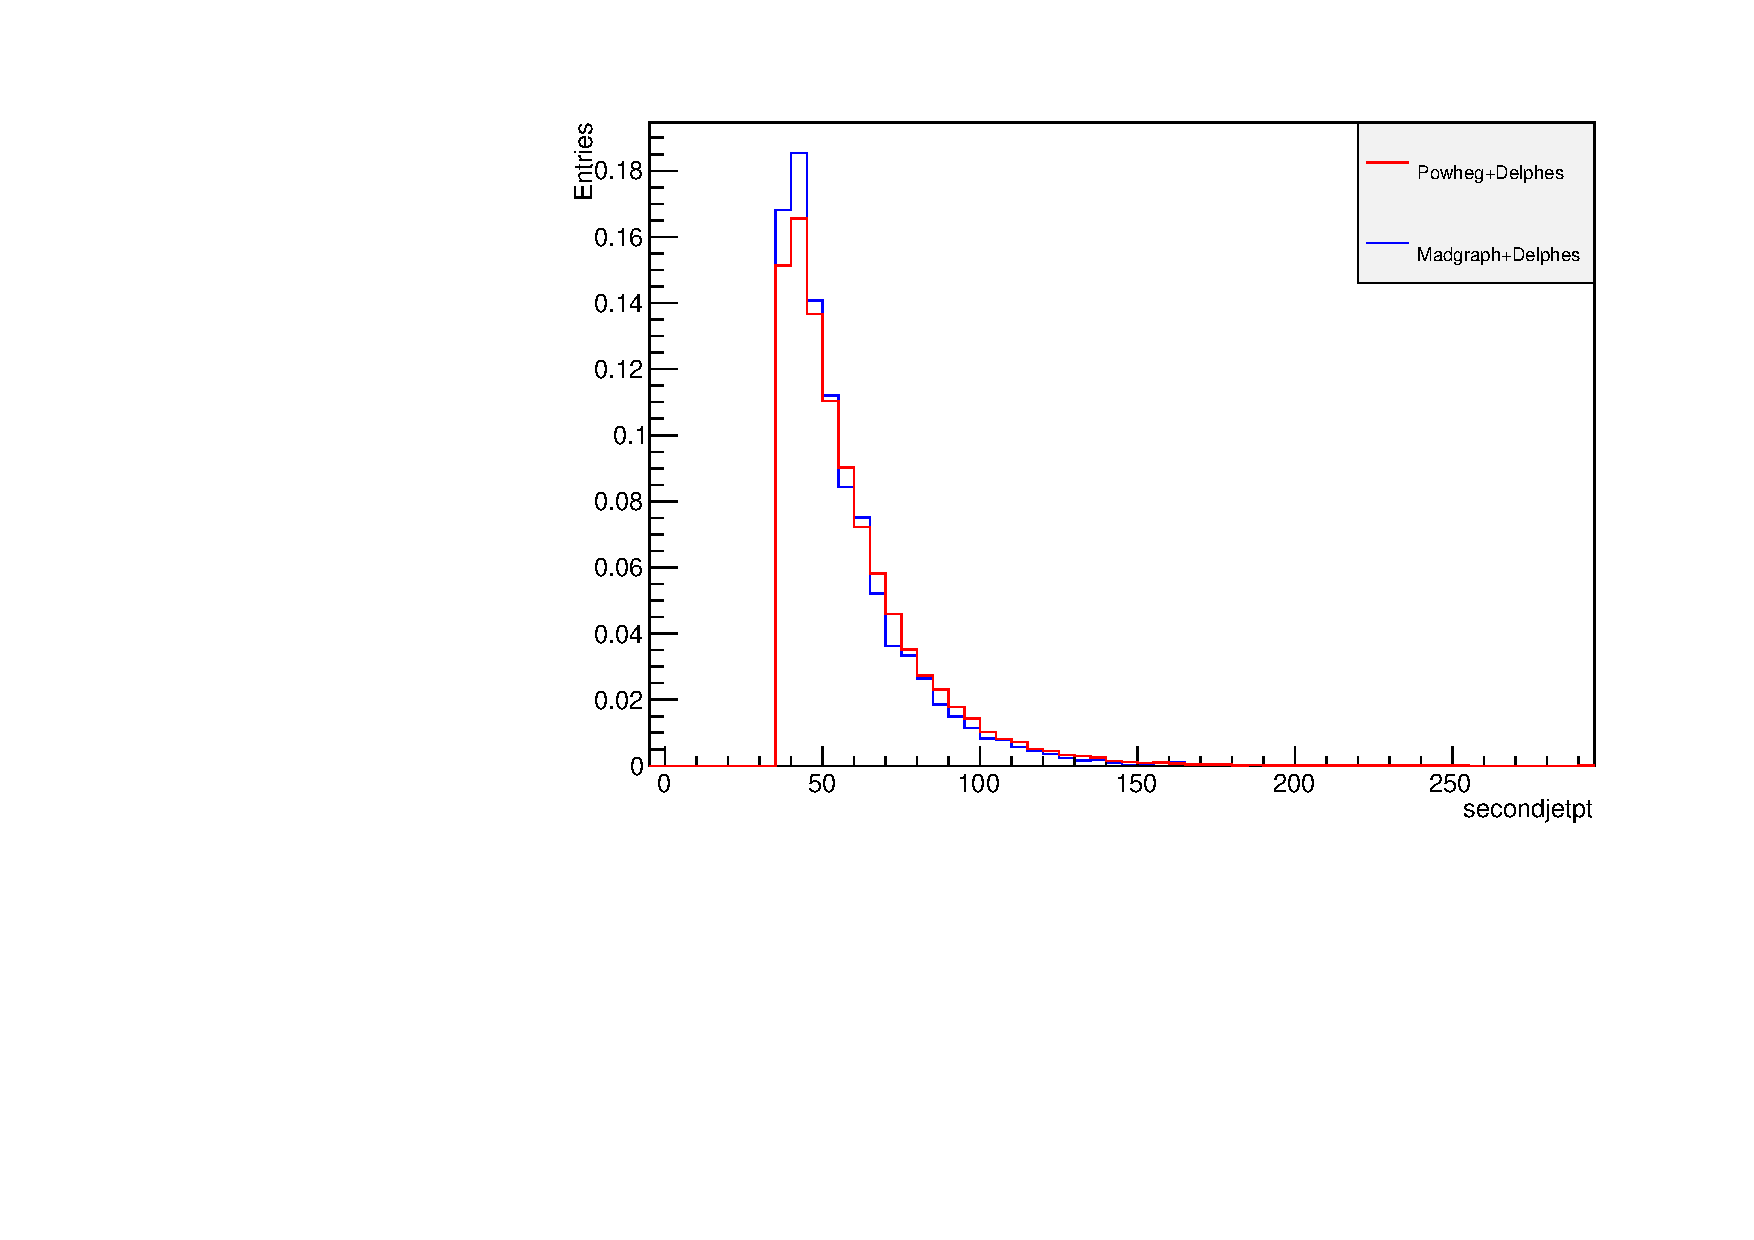
\includegraphics[width=.5\textwidth]{TalkPics/phenoplots221015/secondjetpt_norm.pdf}
    
\end{frame}

\begin{frame}
  \frametitle{Compare Distributions}
  \scriptsize
  \begin{block}{}
    \begin{itemize}
    \item Selection: $\Delta\eta_{jj}>3.6$, jet 1/2 $p_{T}>35$ GeV, trigger MET$>$40 GeV, $\eta_{j1}\cdot\eta_{j2}<0$
    \item Madgraph jets more central than powheg
    \end{itemize}
  \end{block}
  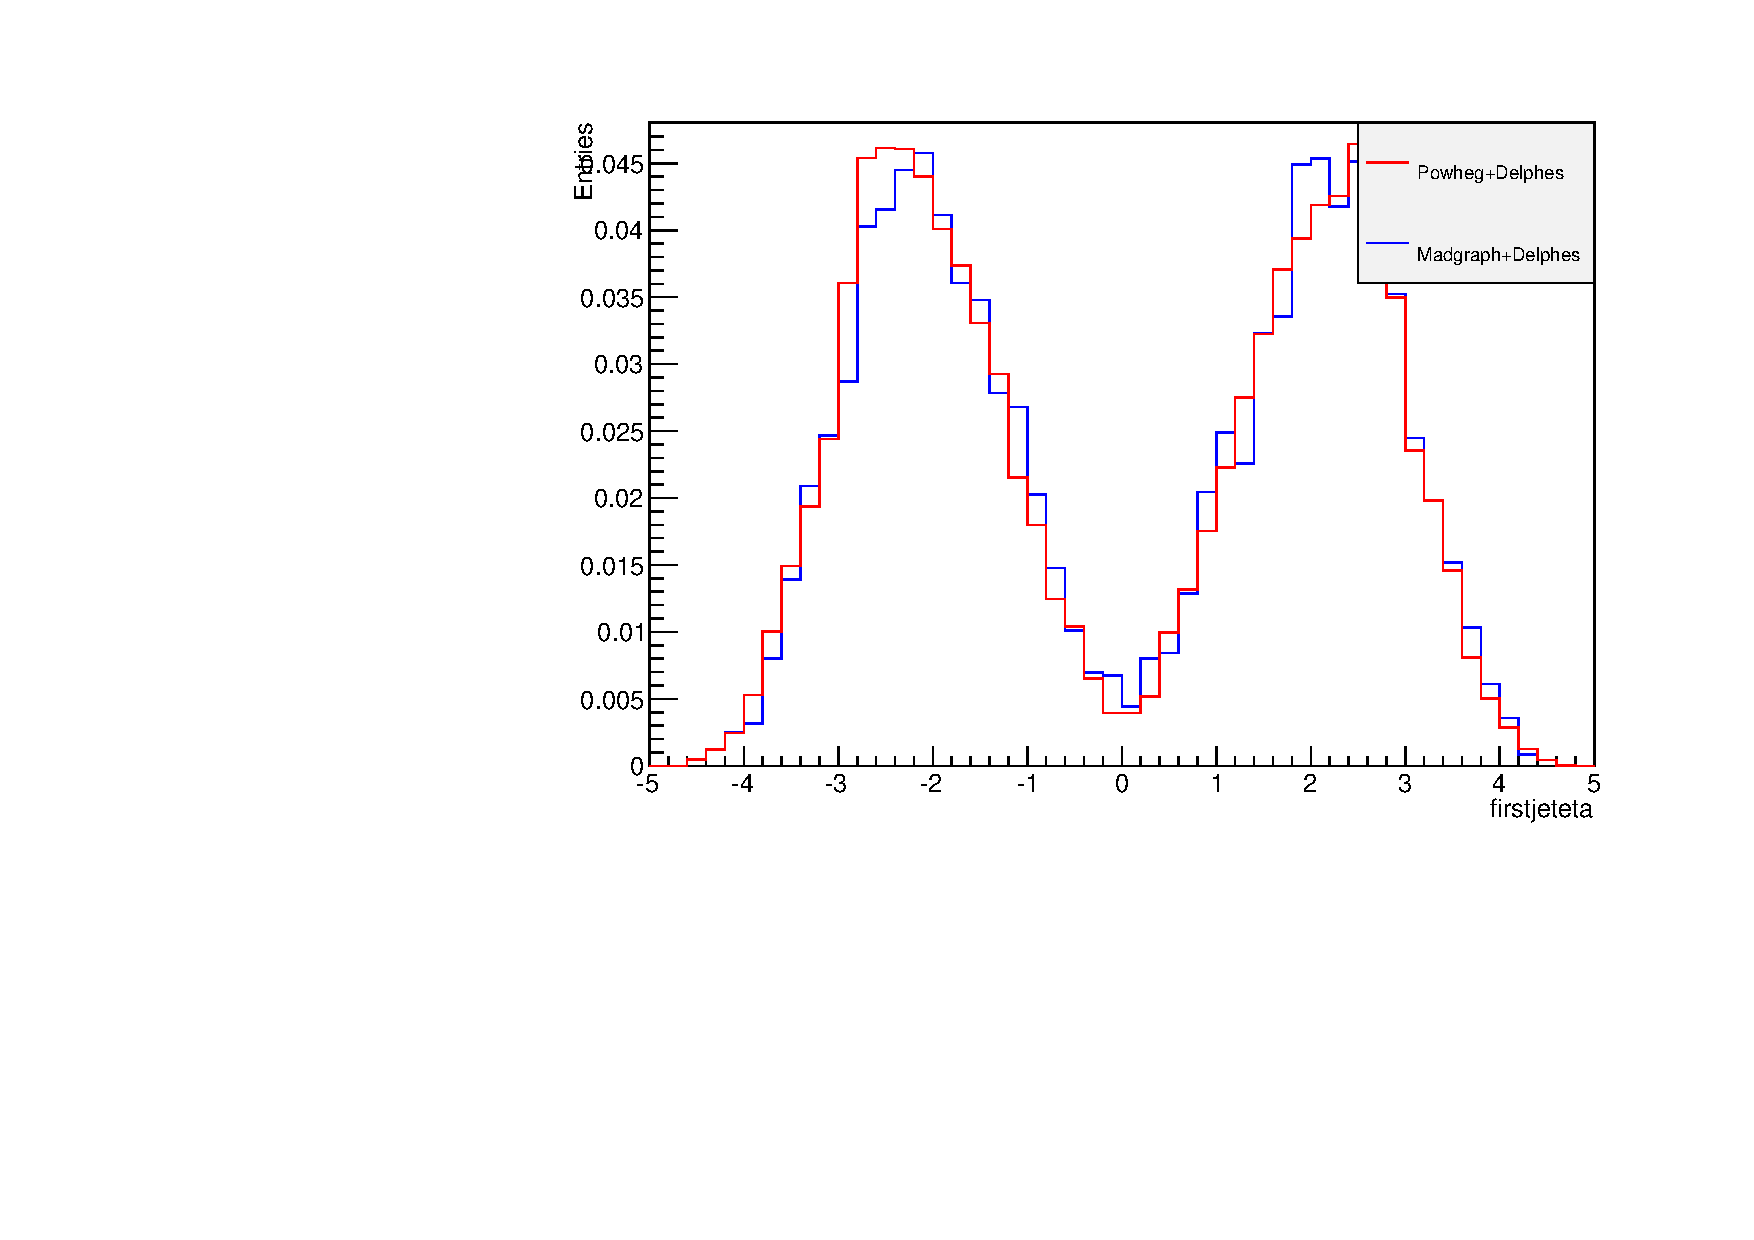
\includegraphics[width=.5\textwidth]{TalkPics/phenoplots221015/firstjeteta_norm.pdf}
  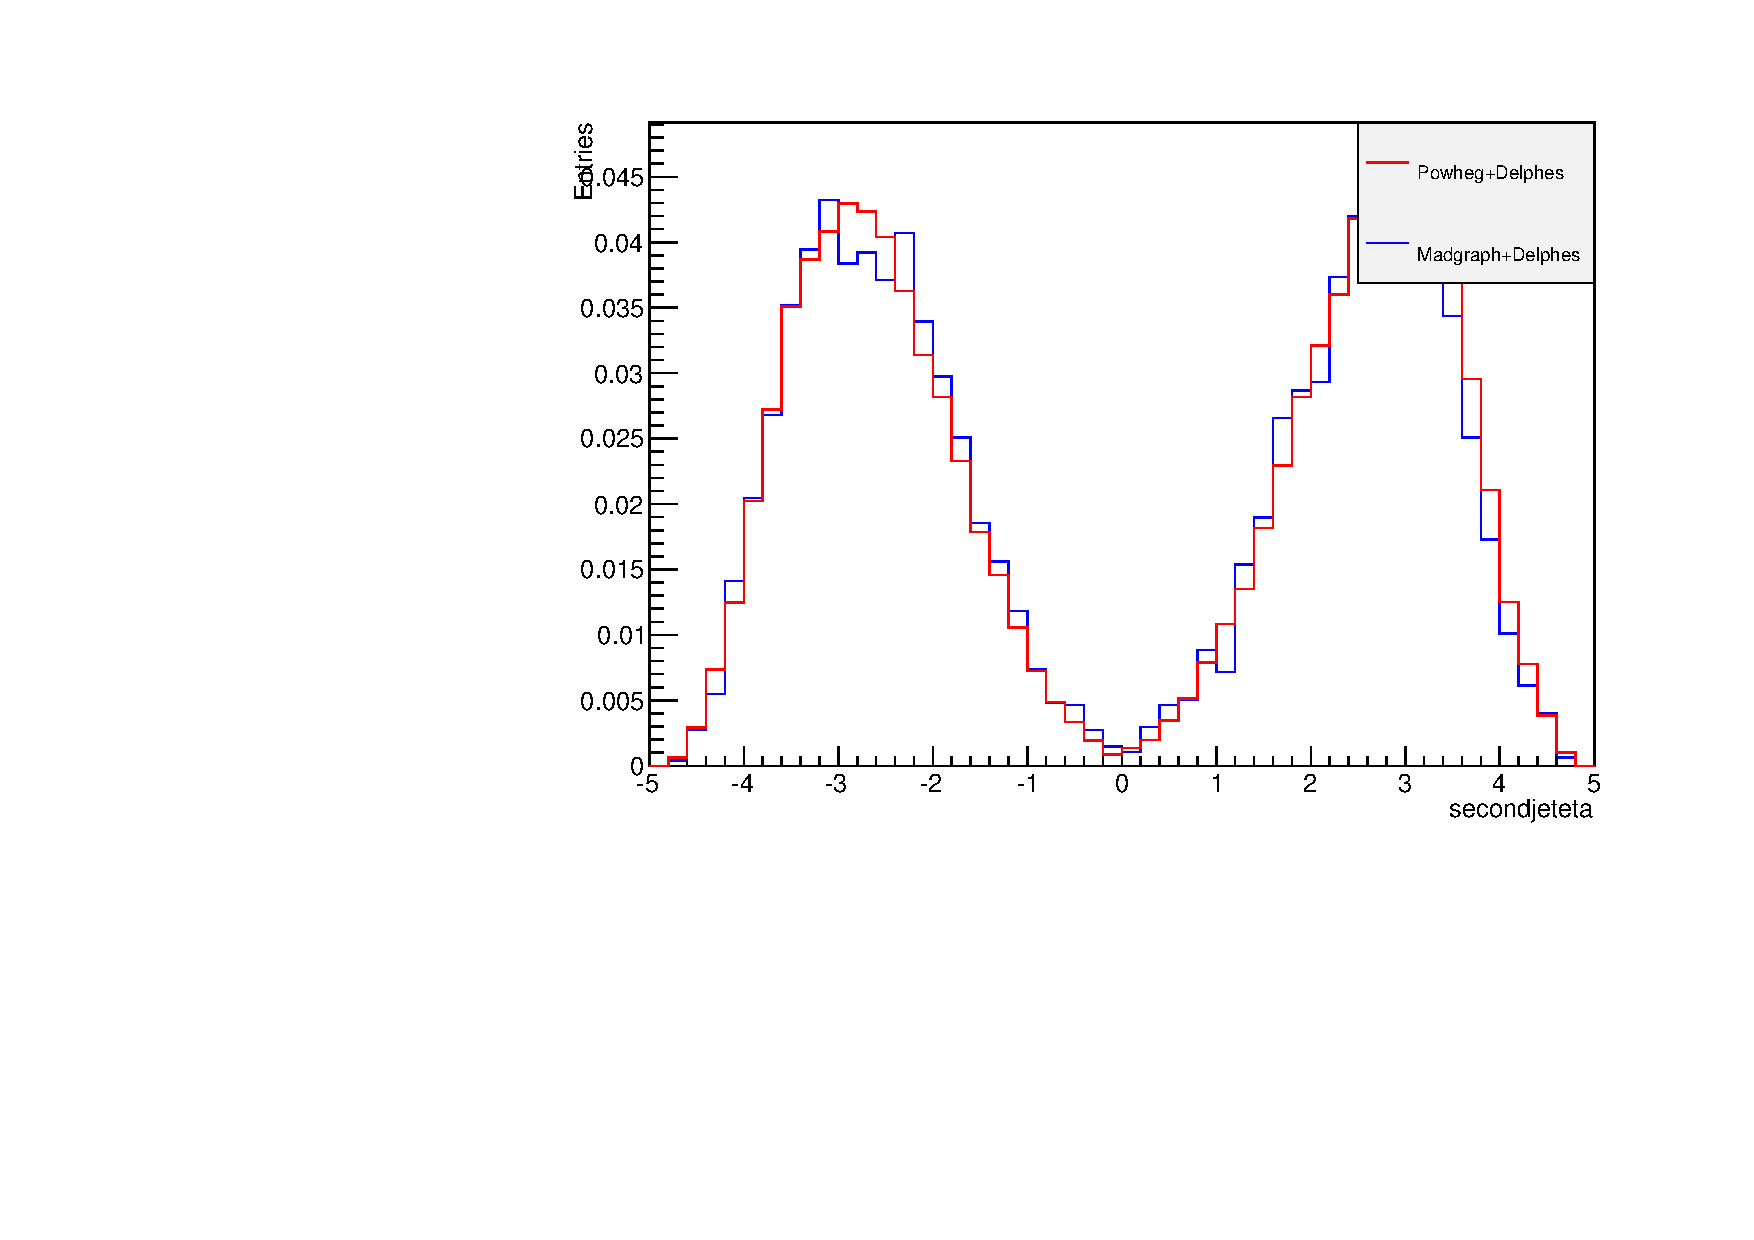
\includegraphics[width=.5\textwidth]{TalkPics/phenoplots221015/secondjeteta_norm.pdf}
    
\end{frame}

\begin{frame}
  \frametitle{Compare Distributions}
  \scriptsize
  \begin{block}{}
    \begin{itemize}
    \item Selection: $\Delta\eta_{jj}>3.6$, jet 1/2 $p_{T}>35$ GeV, trigger MET$>$40 GeV, $\eta_{j1}\cdot\eta_{j2}<0$
    \item Again see madgraph jets being more central
    \item Met a bit lower in madgraph
    \end{itemize}
  \end{block}
  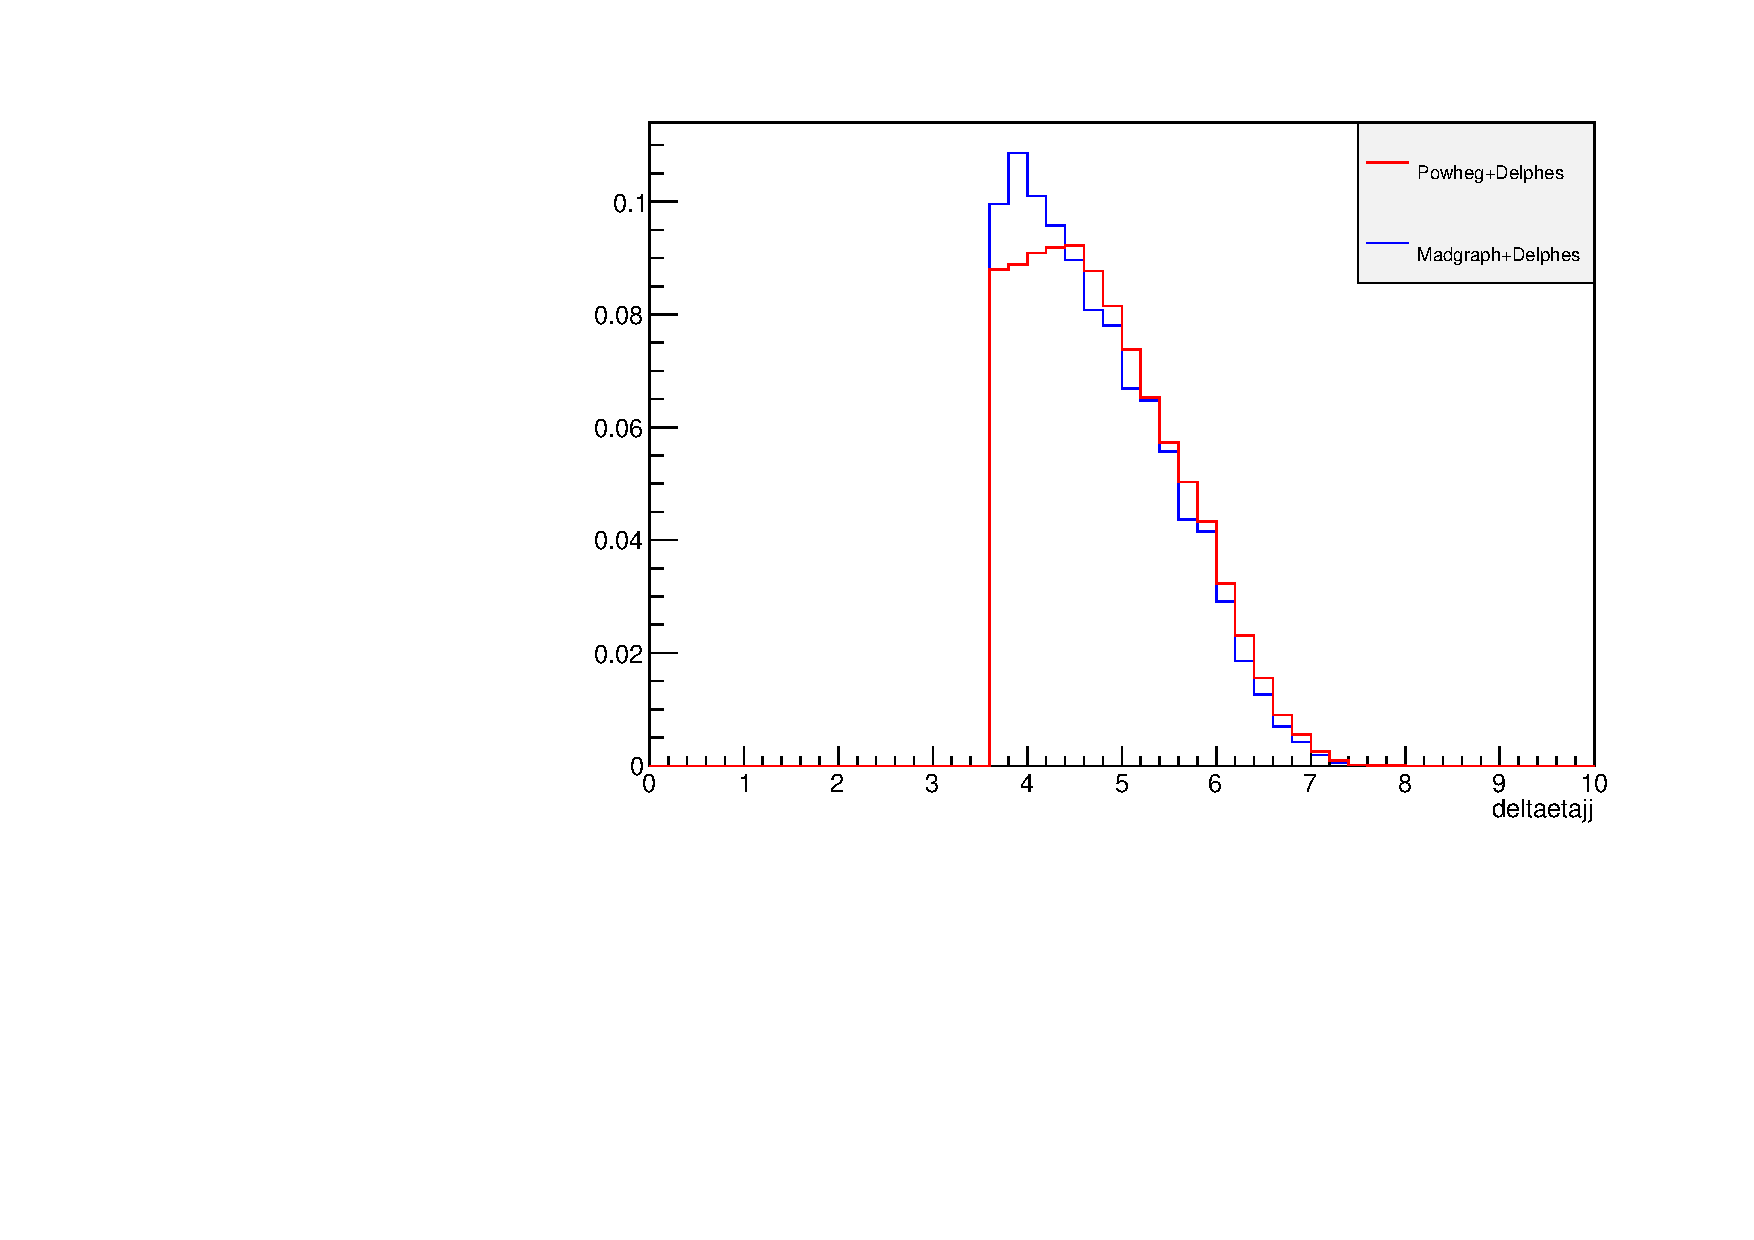
\includegraphics[width=.5\textwidth]{TalkPics/phenoplots221015/deltaetajj_norm.pdf}
  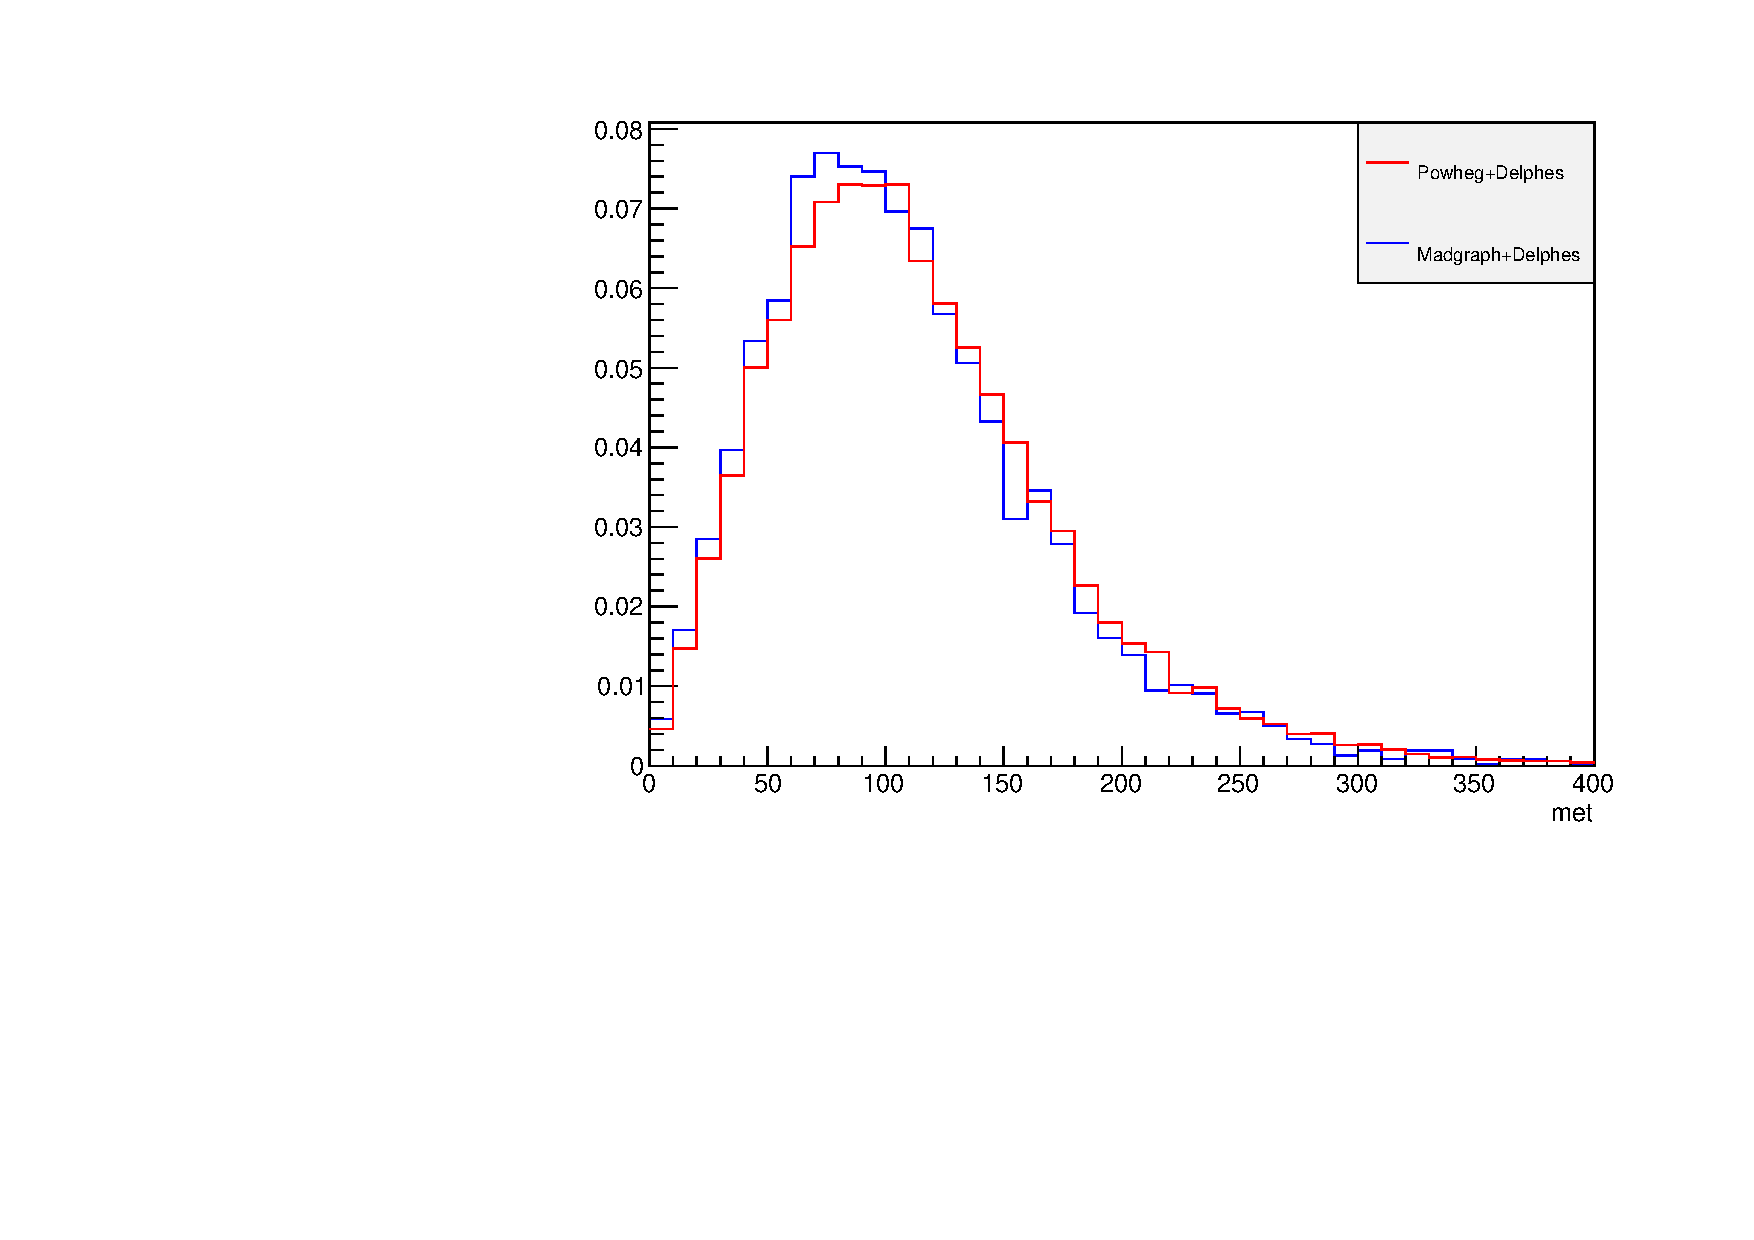
\includegraphics[width=.5\textwidth]{TalkPics/phenoplots221015/met_norm.pdf}
 
\end{frame}

\begin{frame}
  \frametitle{Compare Distributions}
  \scriptsize
  \begin{block}{}
    \begin{itemize}
    \item Selection: $\Delta\eta_{jj}>3.6$, jet 1/2 $p_{T}>35$ GeV, trigger MET$>$40 GeV, $\eta_{j1}\cdot\eta_{j2}<0$
    \item Limited statistics in phi
    \end{itemize}
  \end{block}
  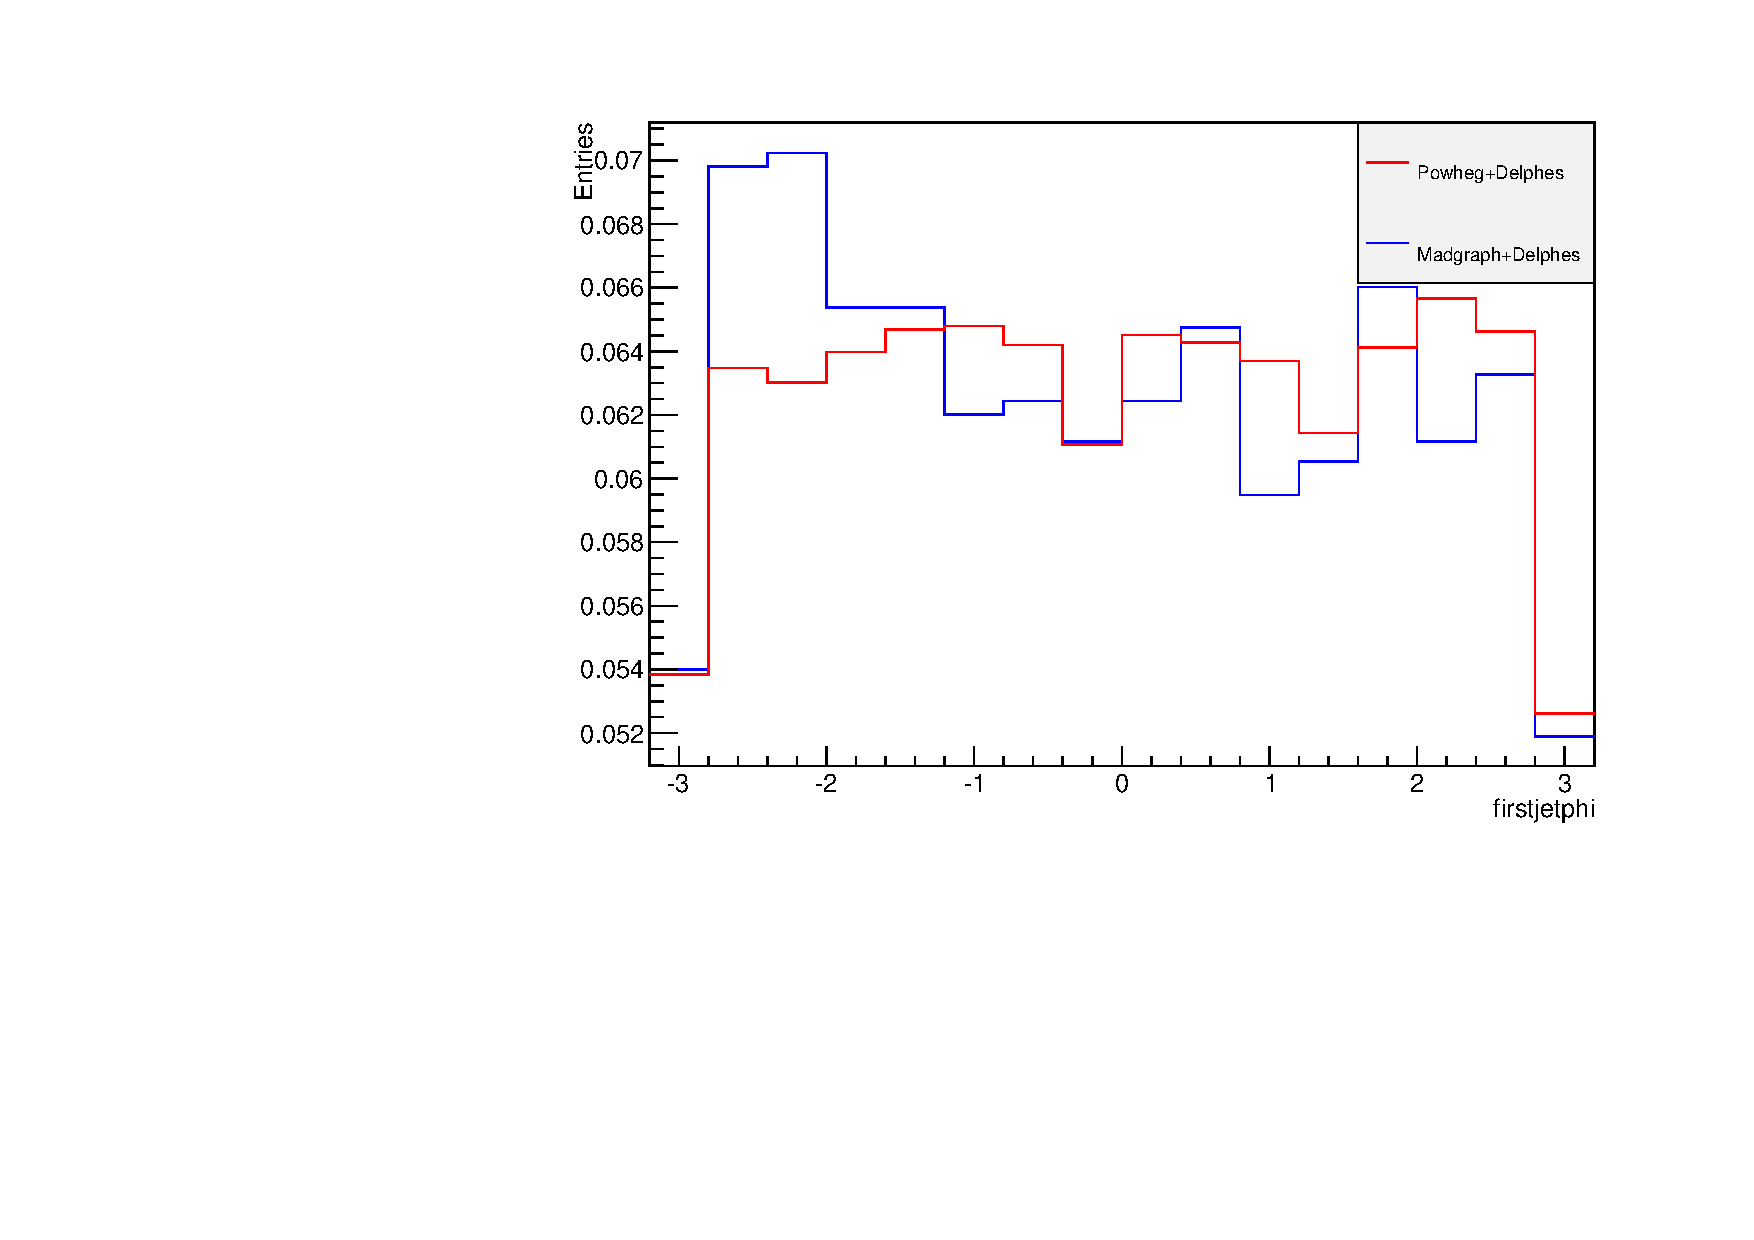
\includegraphics[width=.5\textwidth]{TalkPics/phenoplots221015/firstjetphi_norm.pdf}
  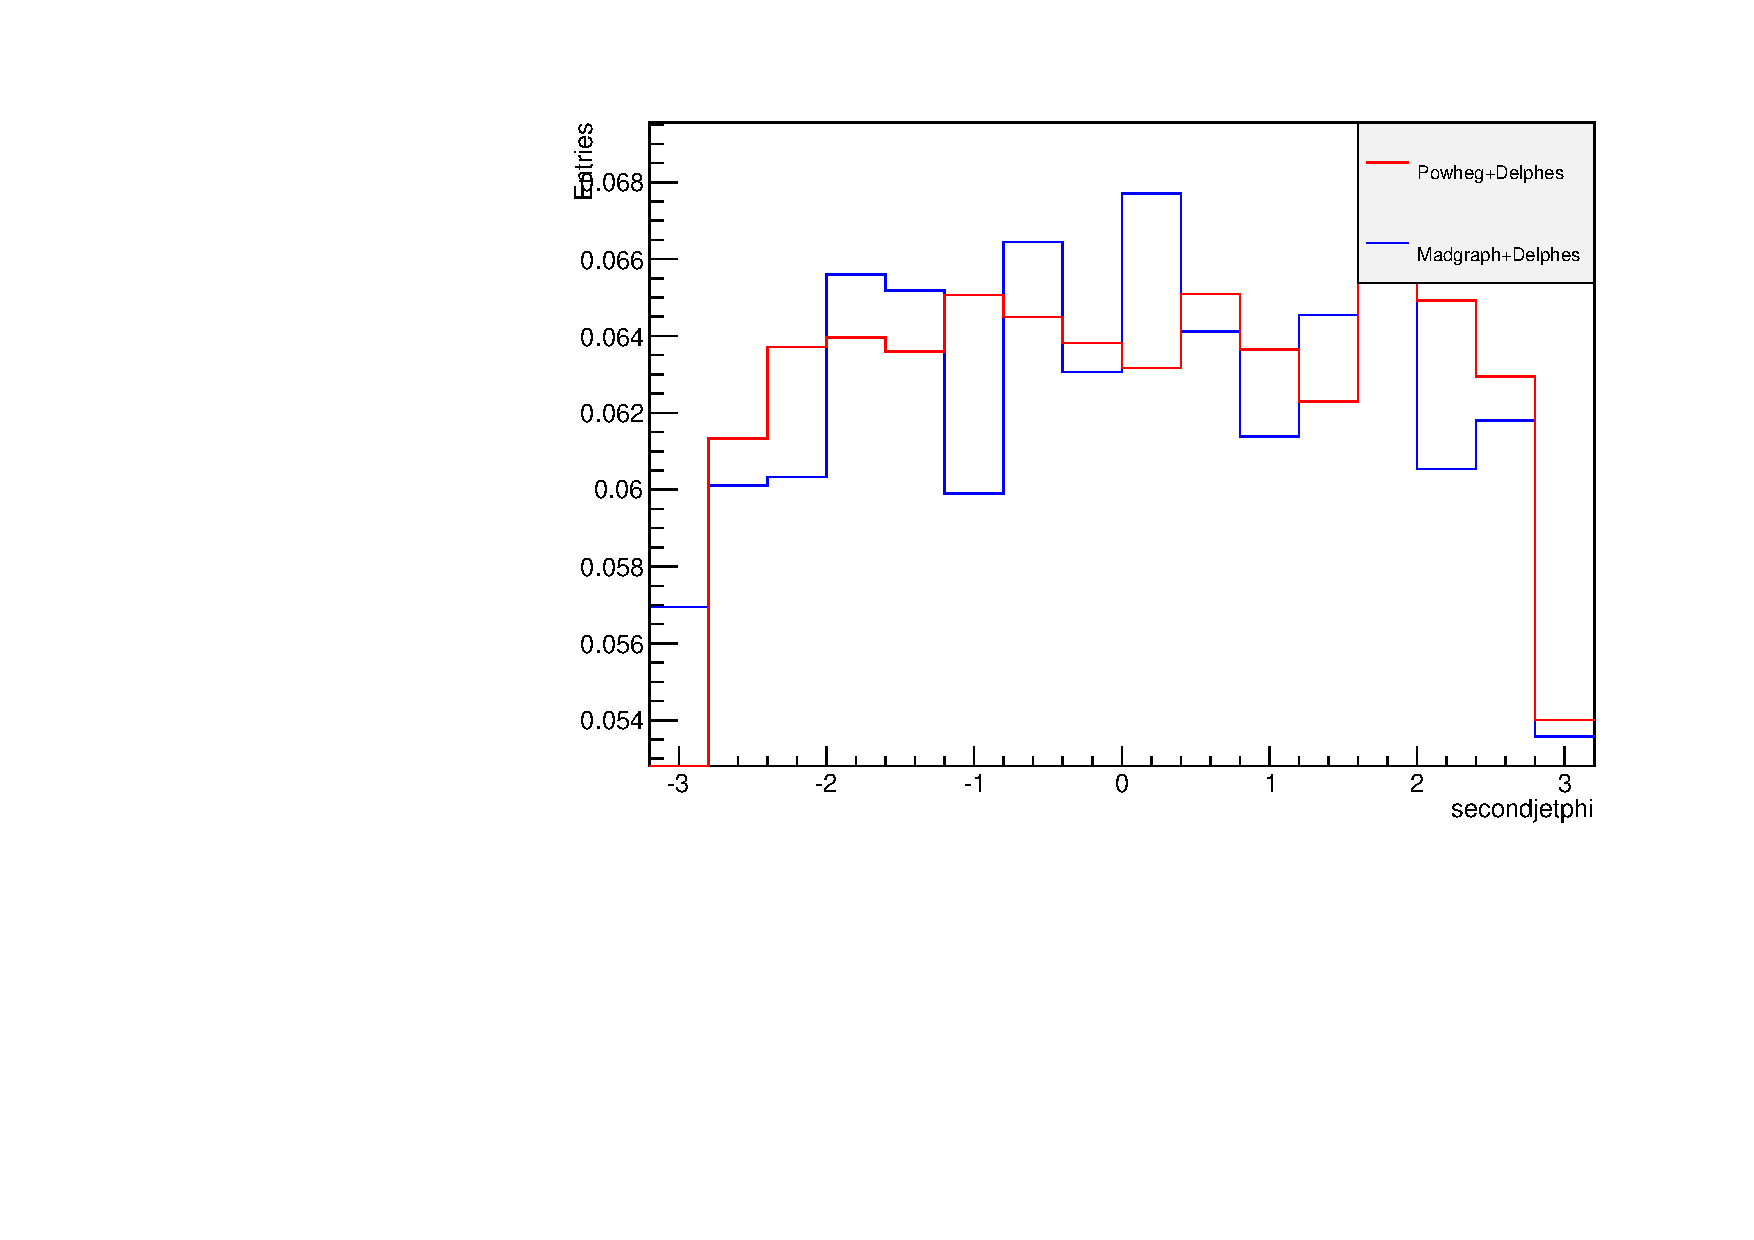
\includegraphics[width=.5\textwidth]{TalkPics/phenoplots221015/secondjetphi_norm.pdf}
    
\end{frame}




\begin{frame}
  \frametitle{Compare Distributions}
  \scriptsize
  \begin{block}{}
    \begin{itemize}
    \item Selection: $\Delta\eta_{jj}>3.6$, jet 1/2 $p_{T}>35$ GeV, trigger MET$>$40 GeV, $\eta_{j1}\cdot\eta_{j2}<0$
    \item More additional jets in madgraph
    \end{itemize}
  \end{block}
  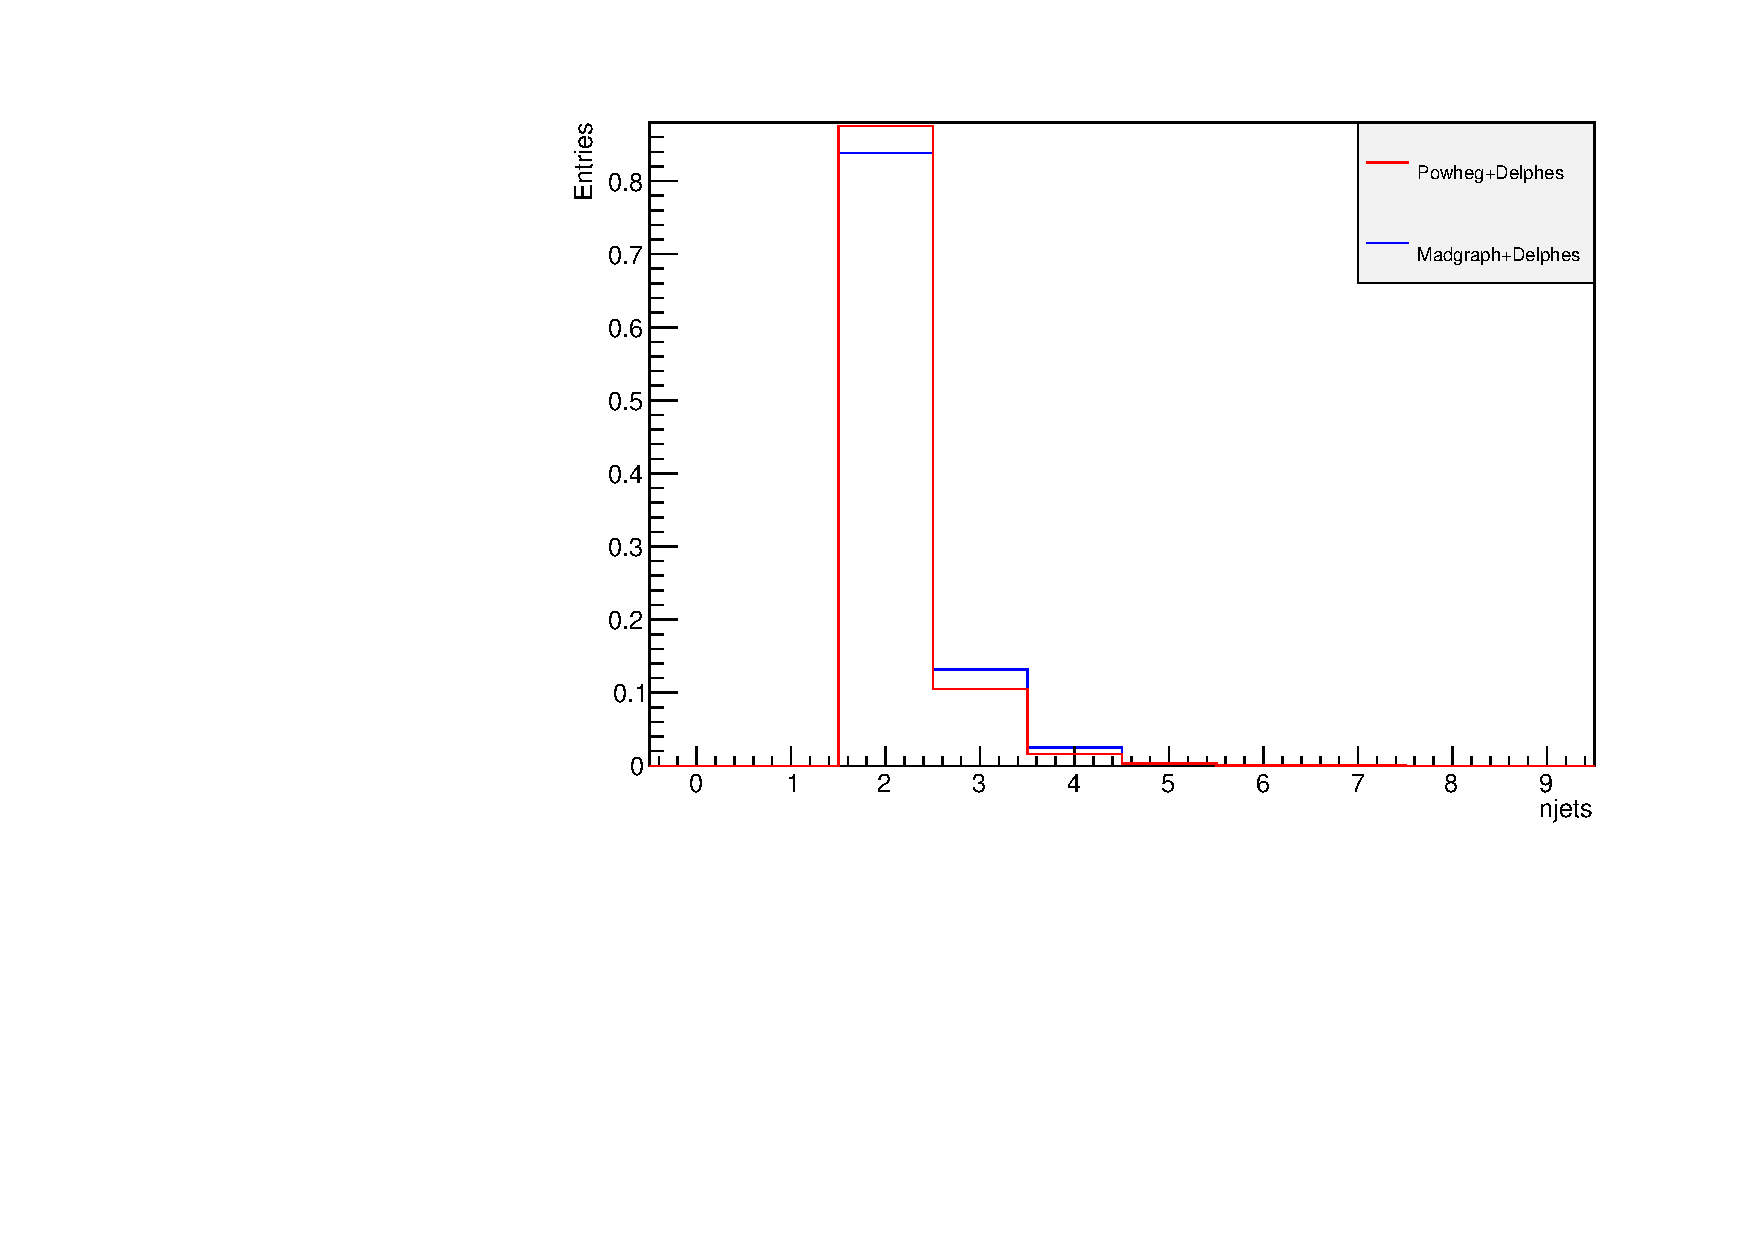
\includegraphics[width=.5\textwidth]{TalkPics/phenoplots221015/njets_norm.pdf}
  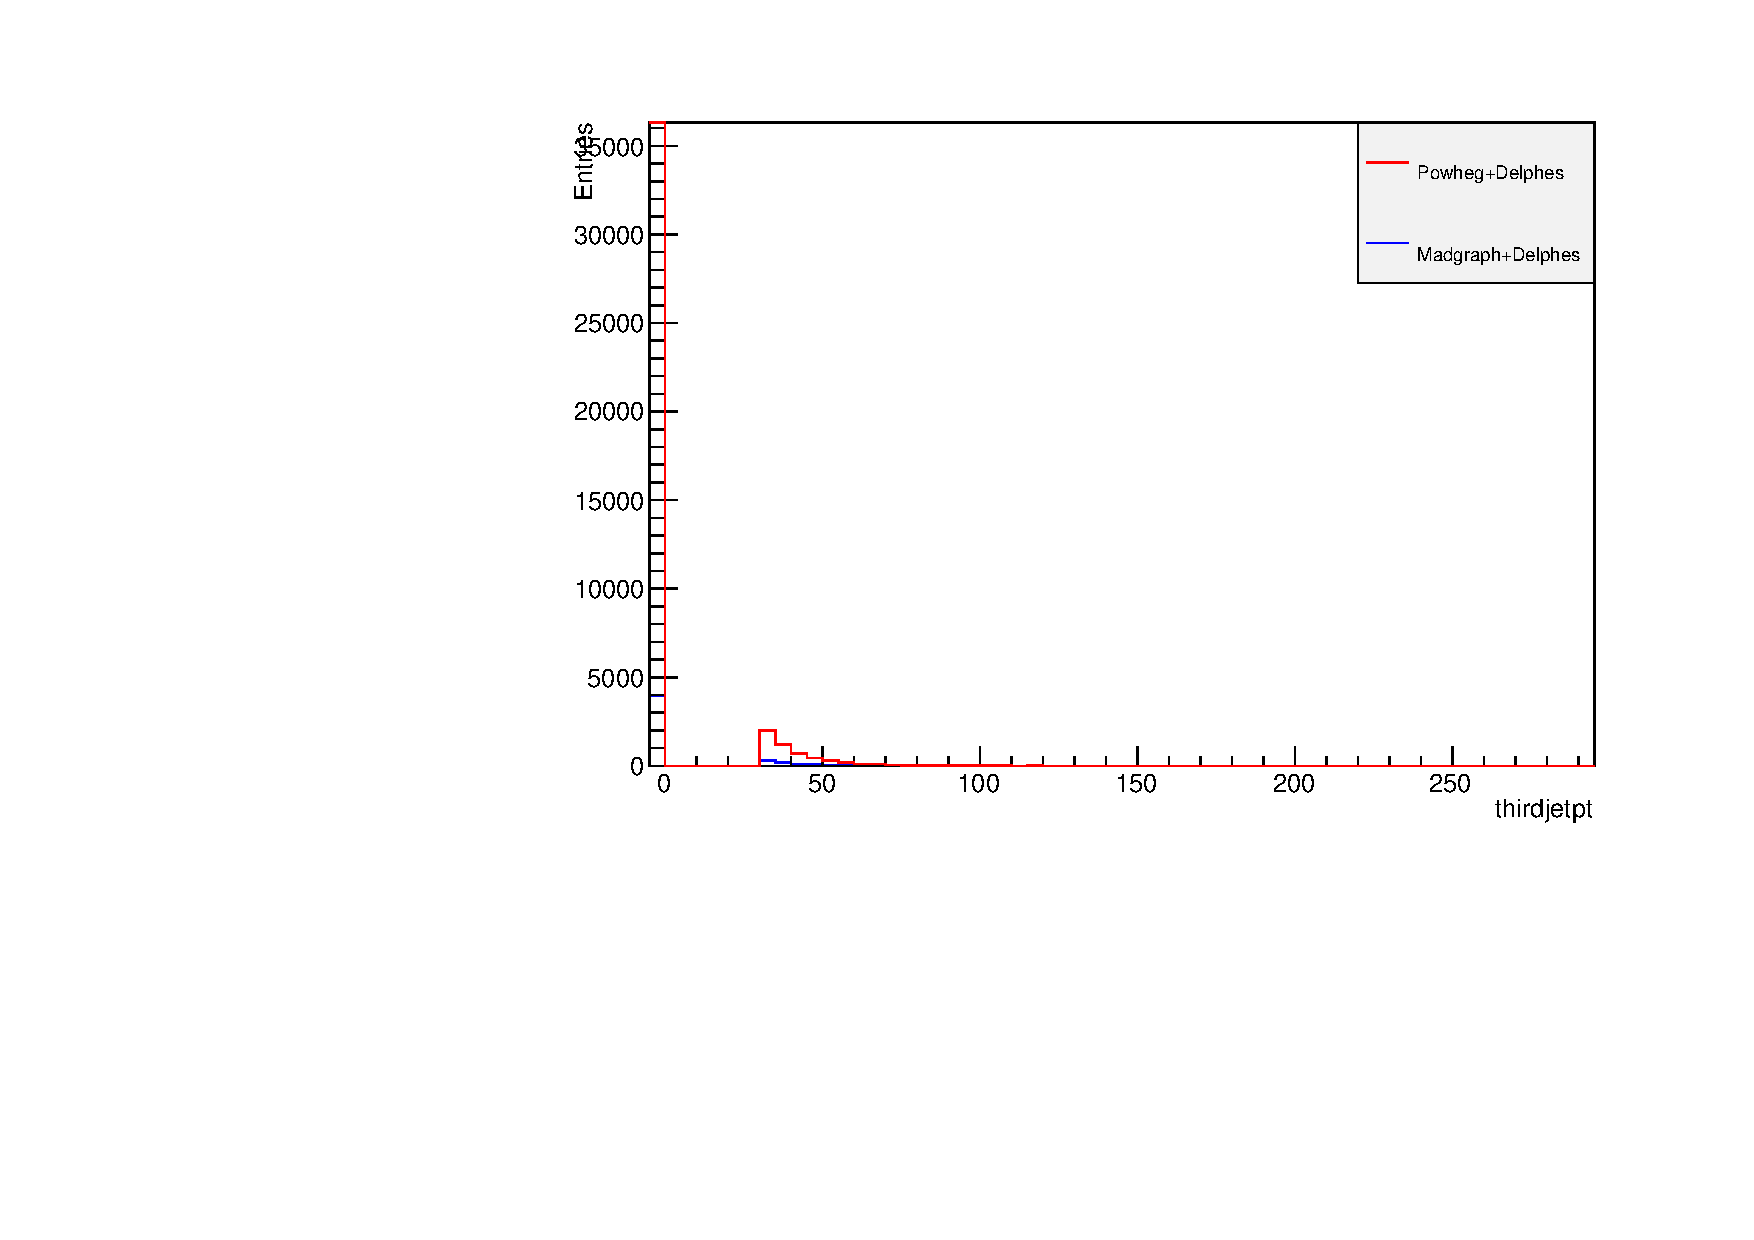
\includegraphics[width=.5\textwidth]{TalkPics/phenoplots221015/thirdjetpt.pdf}
 
    
\end{frame}

\begin{frame}
  \frametitle{Compare Distributions}
  \scriptsize
  \begin{block}{}
    \begin{itemize}
    \item Selection: $\Delta\eta_{jj}>3.6$, jet 1/2 $p_{T}>35$ GeV, trigger MET$>$40 GeV, $\eta_{j1}\cdot\eta_{j2}<0$
    \item More additional jets might make jetmetdphi lower
    \item No difference discernible
    \end{itemize}
  \end{block}
  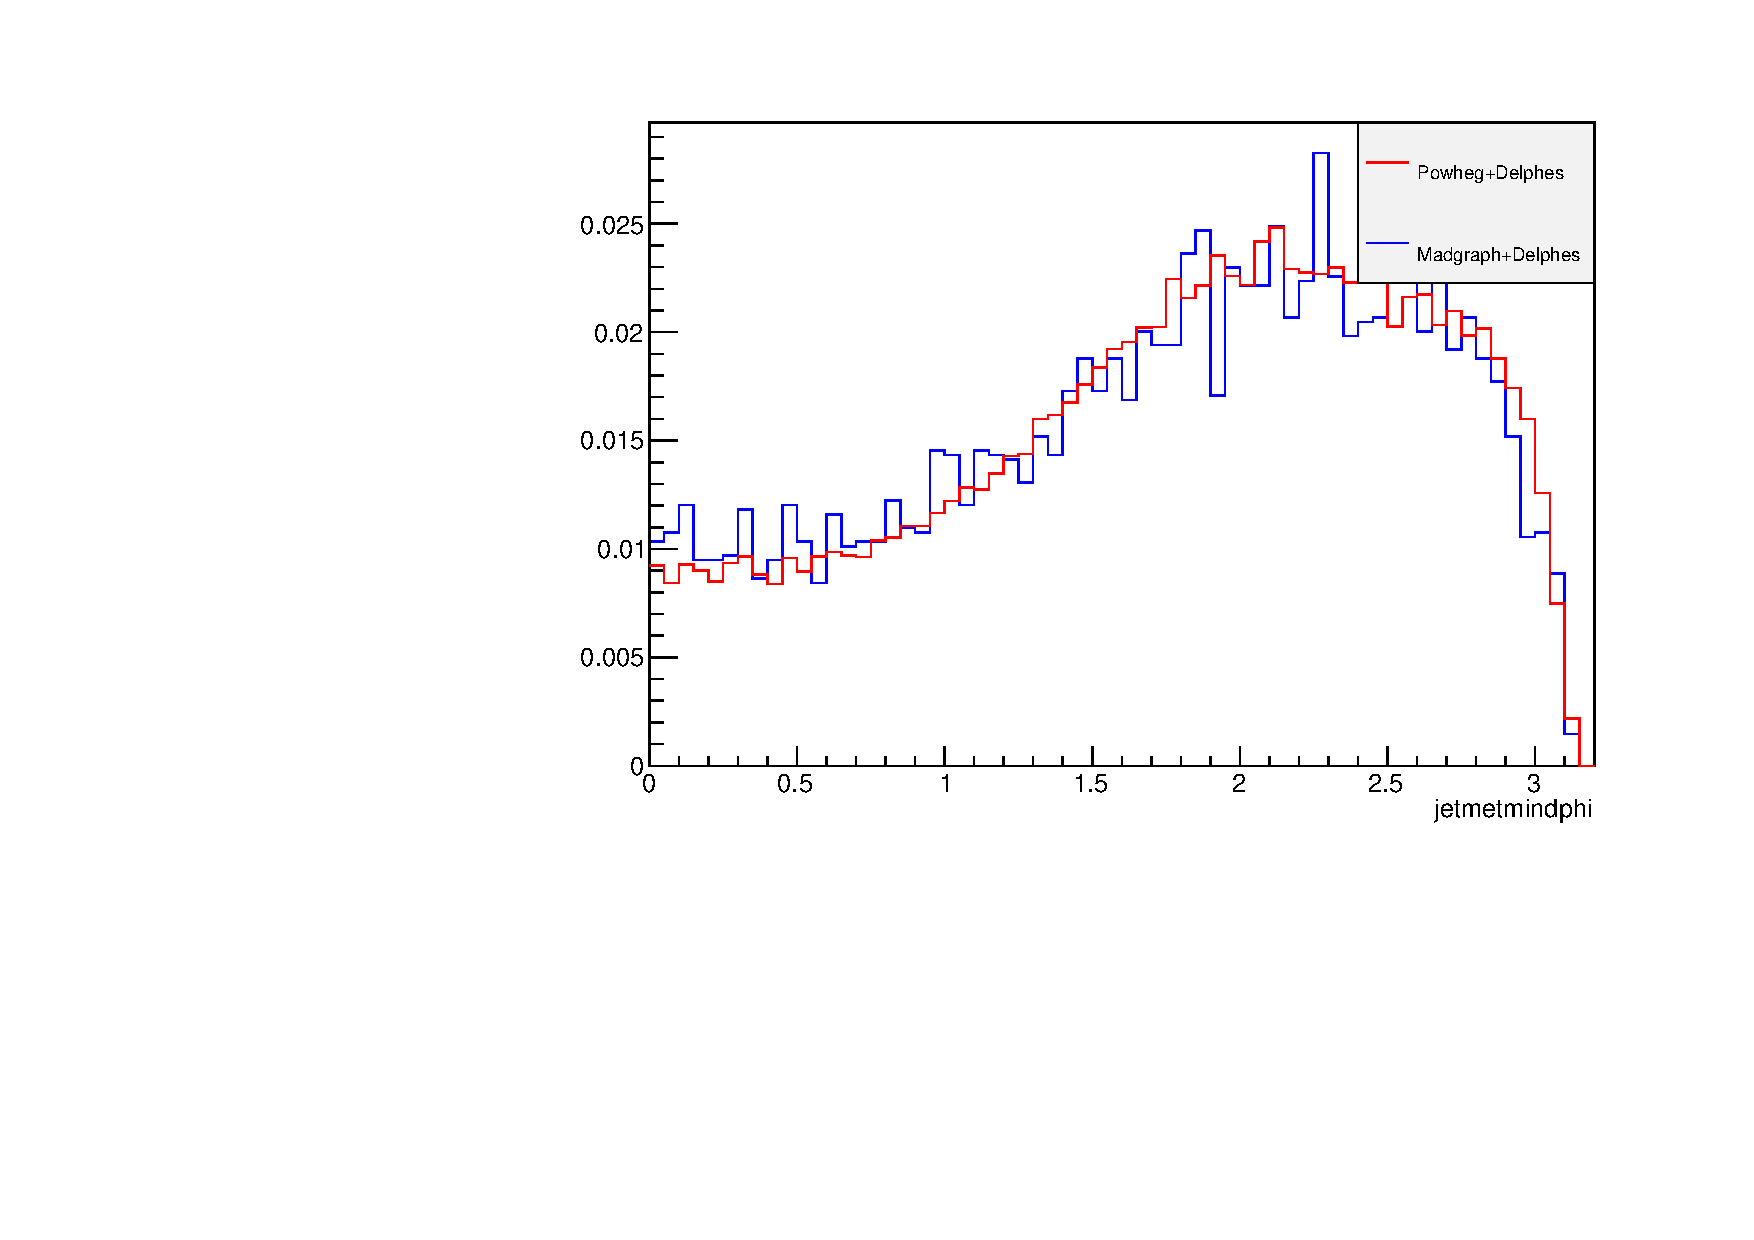
\includegraphics[width=.5\textwidth]{TalkPics/phenoplots221015/jetmetmindphi_norm.pdf}
  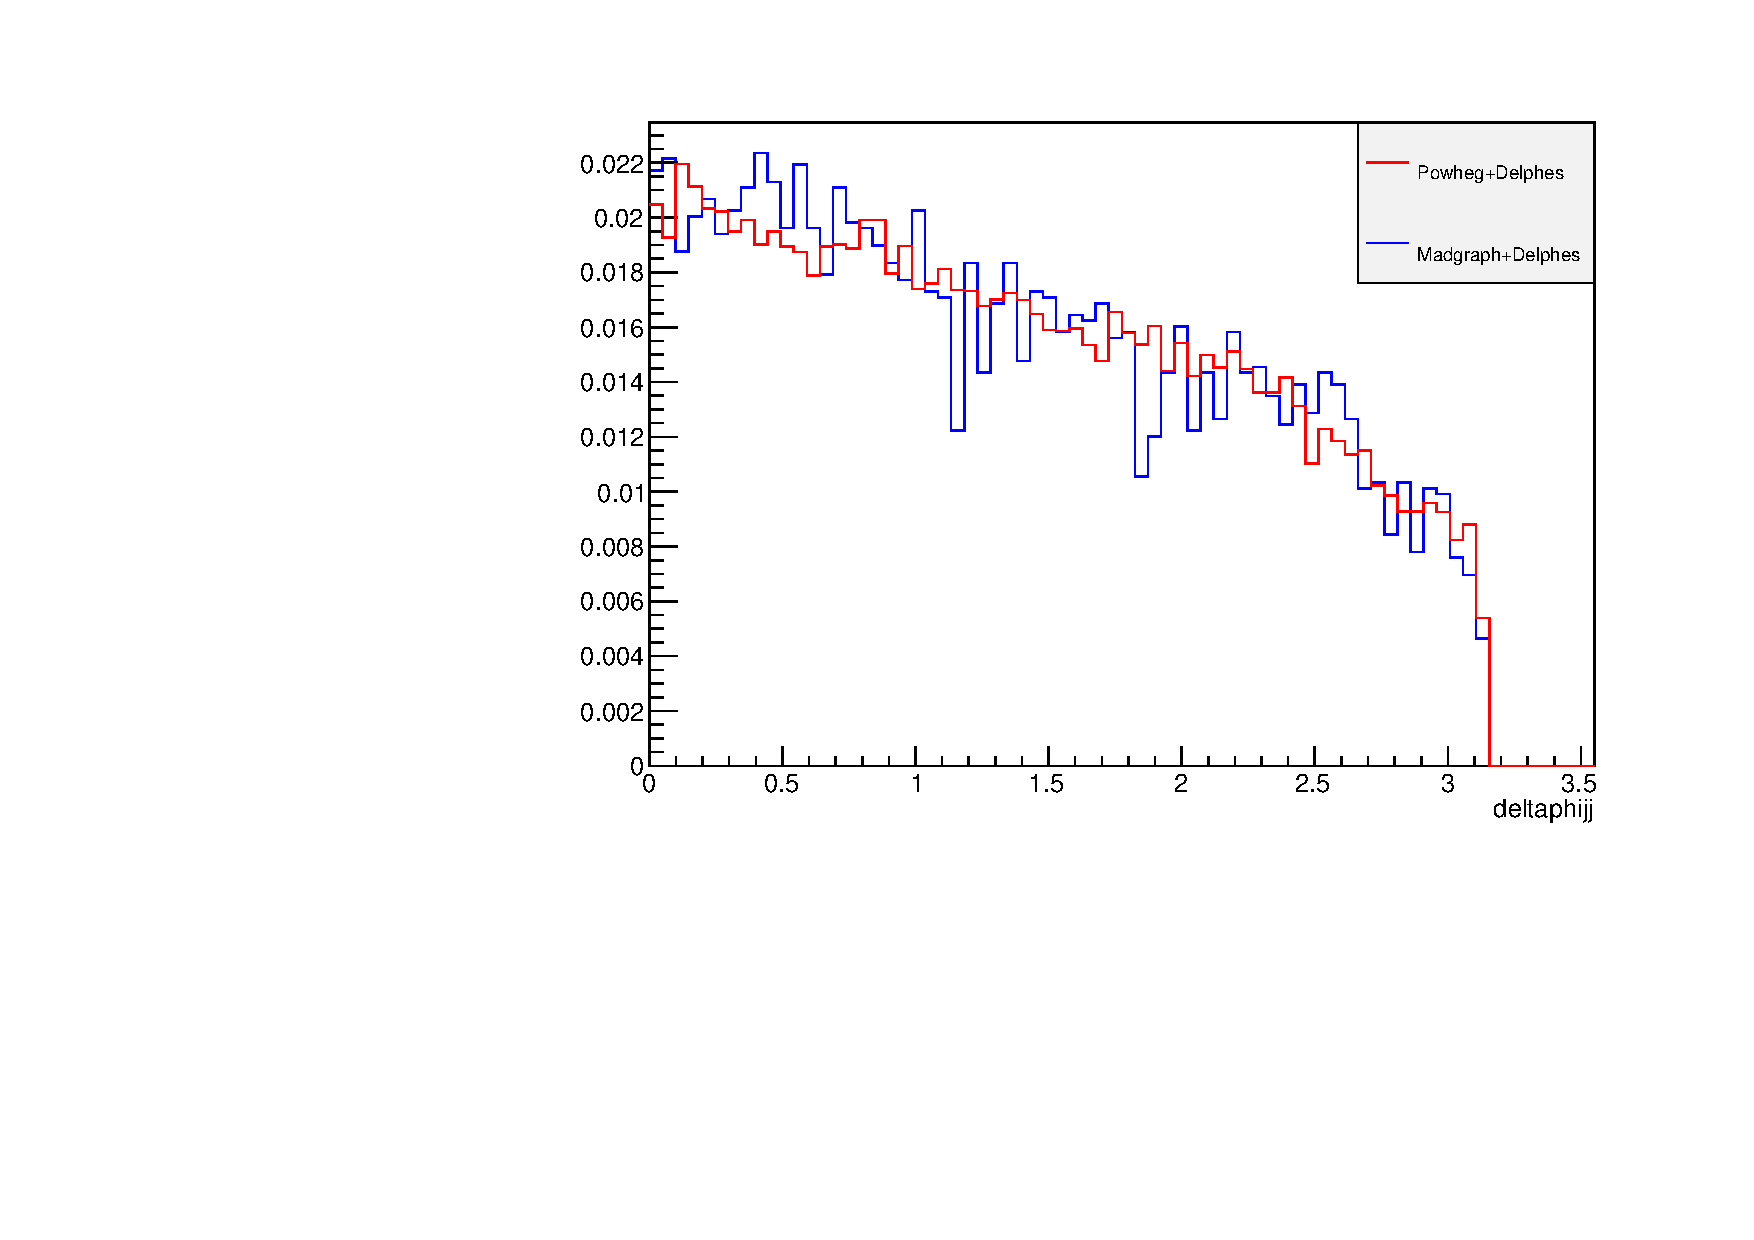
\includegraphics[width=.5\textwidth]{TalkPics/phenoplots221015/deltaphijj_norm.pdf}
 
    
\end{frame}

\begin{frame}
  \frametitle{Summary}
  \label{lastframe}
  \begin{block}{}
    \scriptsize
    \begin{itemize}
    \item We see a factor two difference in final yield between powheg and madgraph
    \item Main effect seems to come from softer $M_{jj}$ and jet $p_{T}$ distributions.
    \end{itemize}
  \end{block}
  \centering
  %!!INCLUDE A RUN 2 PLOT
\end{frame}

%UPDATED BACKUP
\begin{frame}
  \frametitle{Backup}
\end{frame}

\end{fmffile}
\end{document}
